%! suppress = MissingImport
\subsection{Install the \developmentboard\ onto the Breadboard}

    \begin{description}
        \checkoffitem{Orient the breadboard in front of you so that row 1 is on your left and row 63 is on your right;
        column a should be at the bottom, and column j should be at the top.}
        \checkoffitem{\prepunch{\mcuupperrow\ and \mculowerrow}
        See Figure~\ref{fig:prepunching}.}
    \end{description}

    After the paper provides some initial resistance, the jumper's lead will slide into the breadboard's contact point;
    remove the lead and move on to the next contact point.
    You want to pre-punch these holes because the paper provides less resistance when you're inserting a single lead than it does when you're inserting a component with multiple leads.

    \begin{figure}
        \centering
        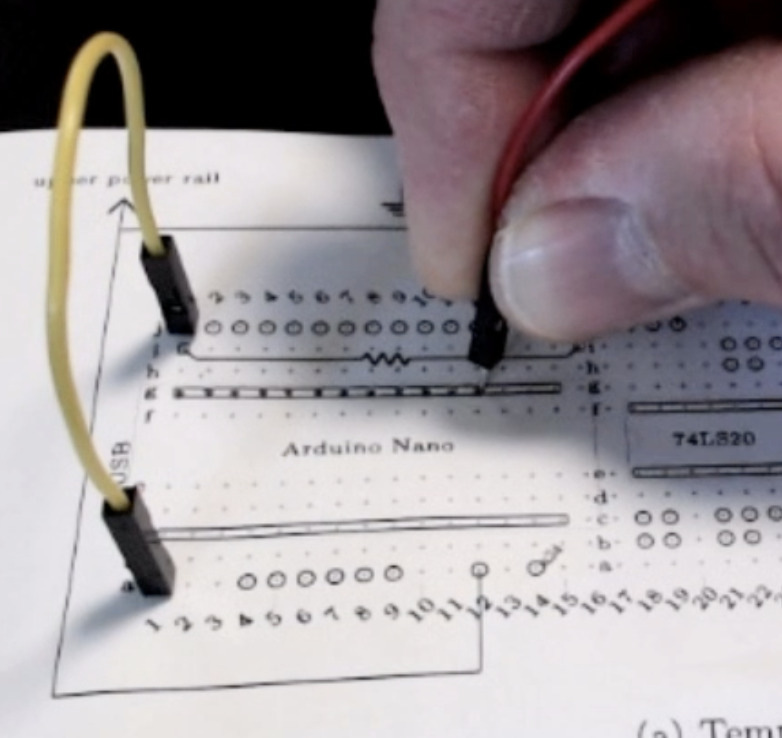
\includegraphics[height=3cm]{microcontroller/breadboard/prepunching}
        \caption{Pre-punching holes in the breadboard template before inserting a component.} \label{fig:prepunching}
    \end{figure}

    \begin{description}
        \checkoffitem{Remove the anti-static foam from the \developmentboard's pins.}
    \end{description}
    You will place the \developmentboard\ on the left side of the breadboard with the USB connector on the left (that is, facing away from the breadboard).
    \begin{description}
        \checkoffitem{Position the upper row of pins on contact points \mcuupperrow\ and the lower row of pins on contact points \mculowerrow.}
    \end{description}
%! suppress = NonMatchingIf
\ifdefstring{\formfactor}{nano}{
    The left side of the \developmentboard\ will obscure the labels for columns c--g.
    The right side of the \developmentboard\ will cover contact points c16--g16 but won't use them.
}{}
\begin{description}
    \checkoffitem{Double-check that:}  % TODO: figure out how to generalize this
        \begin{itemize}
            \item the pin labeled \texttt{D12} is in the upper-left, on contact point g1
            \item the pin labeled \texttt{D13} is in the lower-left, on contact point c1
            \item the pin labeled \texttt{VIN} is in the lower-right, on contact point c15
            \item the pin labeled \texttt{TX1} is in the upper-right, on contact point g15
        \end{itemize}
    \checkoffitem{Gently press on both ends of the \developmentboard\ to insert the pins into the contact points, using a slight rocking motion if necessary (Figure~\ref{fig:inserting-mcu}).}
    \checkoffitem{Press the \developmentboard\ into the breadboard until it physically cannot be inserted any deeper (Figure~\ref{fig:mcu-inserted}).}
\end{description}

%! suppress = NonMatchingIf
\begin{figure}
    \centering
    \subfloat[Press gently on both ends of the \developmentboard.] {
        \ifdefstring{\developmentboard}{Arduino Nano}{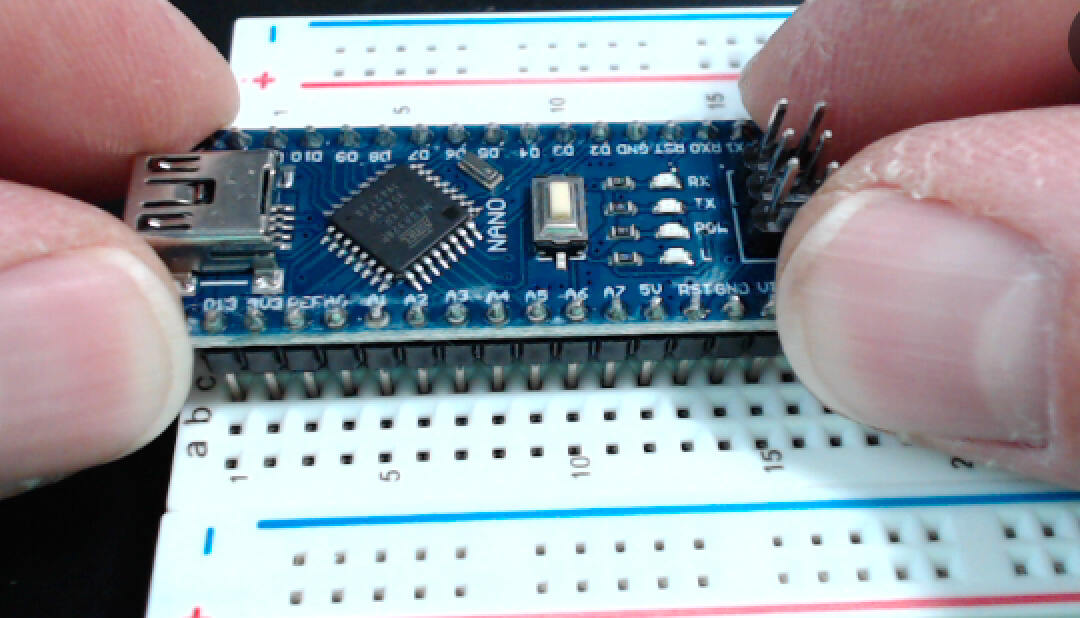
\includegraphics[height=3cm]{microcontroller/breadboard/inserting-nano}}{}
        \label{fig:inserting-mcu}
    }
    \hfil
    \subfloat[The \developmentboard\ fully inserted.] {
        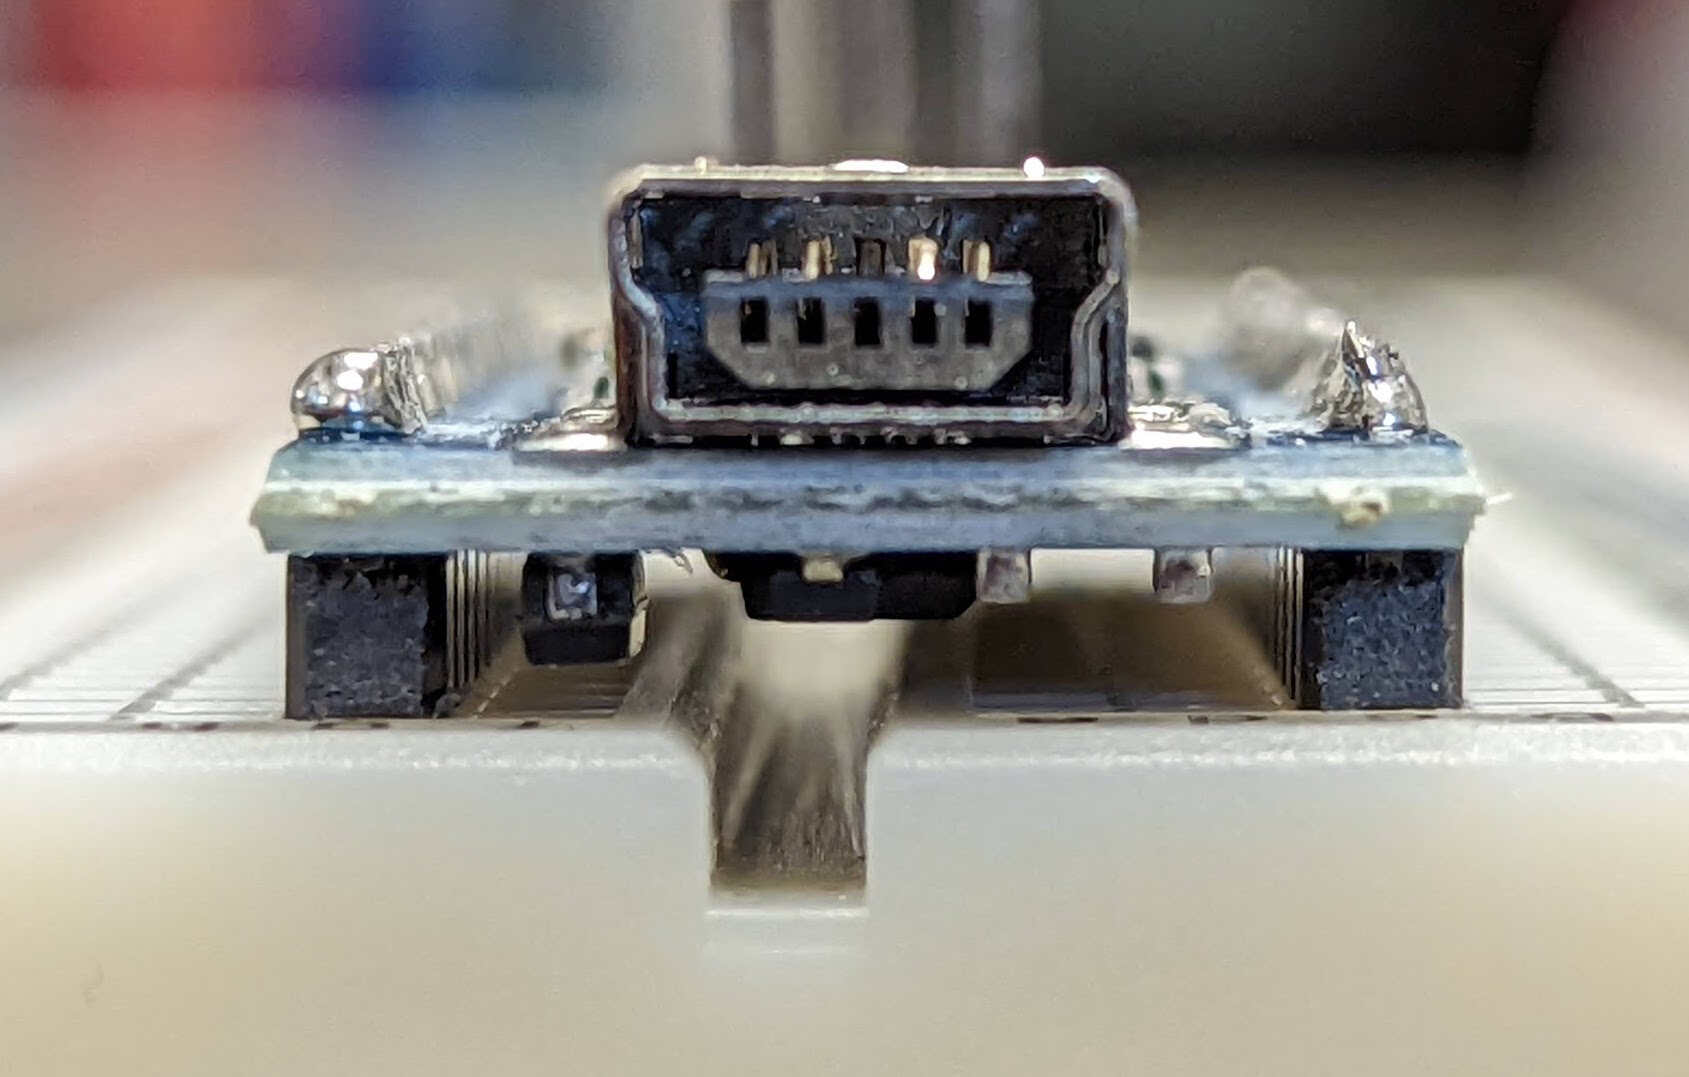
\includegraphics[height=3cm]{microcontroller/breadboard/nano-fully-inserted}
        \label{fig:mcu-inserted}
    }
    \caption{Inserting the \developmentboard\ into the breadboard.}
\end{figure}

\checkpoint{inserted the \developmentboard\ into the breadboard}

\textit{If you are using a breadboard template} then you can now remove the jumper wires from contact points a1 and j1;
the \developmentboard\ will keep the left side of the template pinned in place.
